\chapter{Results}
\label{section:results}

On this section, the results of the multiple experimentation will be given and detailed.

\section{Evaluation Metric}

In task like classification and detection, the research community and also the ActivityNet Challenge use the same metrics for evaluation to be able to compare results between publications. For the classification tasks, for each instance more than one prediction can be made, and for each prediction giving a the probability of success computed. With this multiple predictions for each instance some metric are computed. The simplest one is the \textit{Hit@k}, which gives you the proportion of the instance where the ground truth is on the \textit{top-k} predictions given. For the ActivityNet Challenge $k$ was set to 3.

In addition to this metric, for classifications tasks, it is mostly use the mean Average Precision (mAP) metric. It is computed as the mean of the average precision of all $M$ classes at the Dataset.

\begin{equation}
	mAP = \frac{1}{M} \sum_{m=1}^{M} AP(m)
\end{equation}

At the same time, the Average Precision for each class is computed as the average of the precision at position $n$, showed as $P(n)$. This precision is defined as the amount of elements in $k_m$ between positions 1 and $n$ in the ranked list divided by $n$.

\begin{equation}
	AP(m) = \frac{1}{k_m} \sum_{n=1}^{k_m} P(n)
\end{equation}

For the other task of the Challenge, the temporal localization or detection as the Challenge name it, the metric use to verify the results given is the Intersection Over Union (IoU). This metric compute a prediction as correct if the IoU of the prediction with the ground truth annotations is higher than a value $\alpha$. Then the mAP is computed. For the ActivityNet Challenge the $\alpha$ value used is 0.5.

For all the metrics computations of this section, it has been used the evaluation scripts given by the ActivityNet Challenge 2016 organization.

\section{Classification Task}

The first experiments made were related to the Recurrent Neural Network architecture, in order to obtain the best performance. The way to measure the performance, was computing the mAP for the classification task. The different architectures first tested were related to the deep of the network. On the first experiment, it was tested from a 3 layers LSTM with 1024 cells each layer, to a one single layer with 512 cells, going through a two layers network with 512 LSTM cells each one. All the architectures presented a batch normalization after the input entrance and dropout before and after the LSTM layers. Also all the experiments were done exclusively with the features extracted from the C3D network.

As is showed on Table~\ref{table:classification_by_architecture}, the network that achieved the best performance was achieved with the simplest one as was expected while training due to the fact that all the networks presented high learning capacity over our data.

\begin{table}[H]
\begin{center}
\begin{tabular}{|l|c|c|}
\hline
Architecture & mAP & Hit@3 \\
\hline\hline
3 x 1024-LSTM & 0.5635 & 0.7437 \\
2 x 512-LSTM & 0.5492 & 0.7364 \\
1 x 512-LSTM & \bf0.5938 & \bf0.7576 \\
\hline
\end{tabular}
\end{center}
\caption{Results for classification task comparing different deep architectures. All values with
         only video features on the validation dataset.}
\label{table:classification_by_architecture}
\end{table}

Once the best architecture was chosen in the sense of deepness, the network was trained comparing the input features used and also comparing the basic architecture with the one that feedback from the previous output. On the Table~\ref{table:classification_by_features} can be seen how the basic architecture and with only features from the video obtain the best results.

\begin{table}[H]
\begin{center}
\begin{tabular}{|l|c|c|}
\hline
Features used & mAP & Hit@3 \\
\hline\hline
Only video & \bf0.5938 & \bf0.7576 \\
Video w/ audio & 0.5755 & 0.7352 \\
Only video \& feedback & 0.5210 & 0.6982 \\
Video w/ audio \& feedback & 0.5652 & 0.7319 \\
\hline
\end{tabular}
\end{center}
\caption{Results for classification task with the model made by one 512-LSTM. Compare between
         features and feedback on the validation dataset.}
\label{table:classification_by_features}
\end{table}

%%%%%%
How I justify that with audio features the results are worst?
%%%%%%

The ActivityNet Dataset offers a 200 activities videos, but all this activities come from a taxonomy with hierarchically activities. The 200 activities which are annotated all the videos of the dataset and the proposed network predict are the leaf nodes of the taxonomy tree. On this structure there is 5 top level categories which all the videos belongs and describe more generally the activity happening on the video. These are: \textit{Eating and drinking activities}, \textit{Sports, Exercise and Recreation}, \textit{Household Activities}, \textit{Socializing, Relaxing and Leisure}, \textit{Personal Care}.

For all these top level activities, the mean average precision has been computed. To do so, all the predicted and ground truth activity labels have been changed by its top level activity and then for each of them computed the Average Precision. As can be seen on Table~\ref{table:top_level_classification_ap} and Figure~\ref{table:top_level_classification_ap} the \textit{Sports, Exercise and Recreation} have an average precision of $94\%$. This can be explained with the fact that all the features extracted from the videos come from a network which weights were trained to work with a dataset of videos, the Sports1M\cite{KarpathyCVPR14}.

\begin{table}[H]
\begin{center}
\begin{tabular}{|r|c|}
\hline
\textbf{Global Activities} & \textbf{AP} \\
\hline\hline
Eating and drinking Activities & 0.56942 \\
Sports, Exercise, and Recreation & 0.93662 \\
Household Activities & 0.74177 \\
Socializing, Relaxing, and Leisure & 0.76494 \\
Personal Care & 0.59931 \\
\hline\hline
\textbf{Global} (mAP) & 0.72241 \\
\textbf{Global} (Hit@3) & 0.92703 \\
\hline
\end{tabular}
\end{center}
\caption{Mean Average Precision computed for the top level activities of the ActivityNet Dataset. The results are computed over the validation dataset.}
\label{table:top_level_classification_ap}
\end{table}

\begin{figure}[H]
\begin{center}
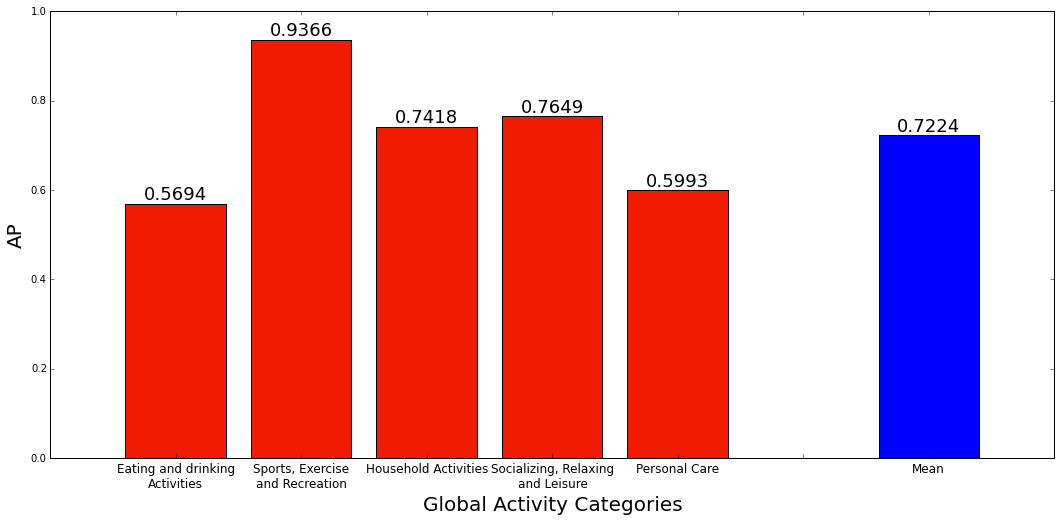
\includegraphics[width=1\linewidth]{img/results/top_activities_classification_ap}
\end{center}
\caption{Representation of the results over the top-level activities}
\label{fig:top_level_classification_ap}
\end{figure}



\begin{figure}[H]
\begin{center}
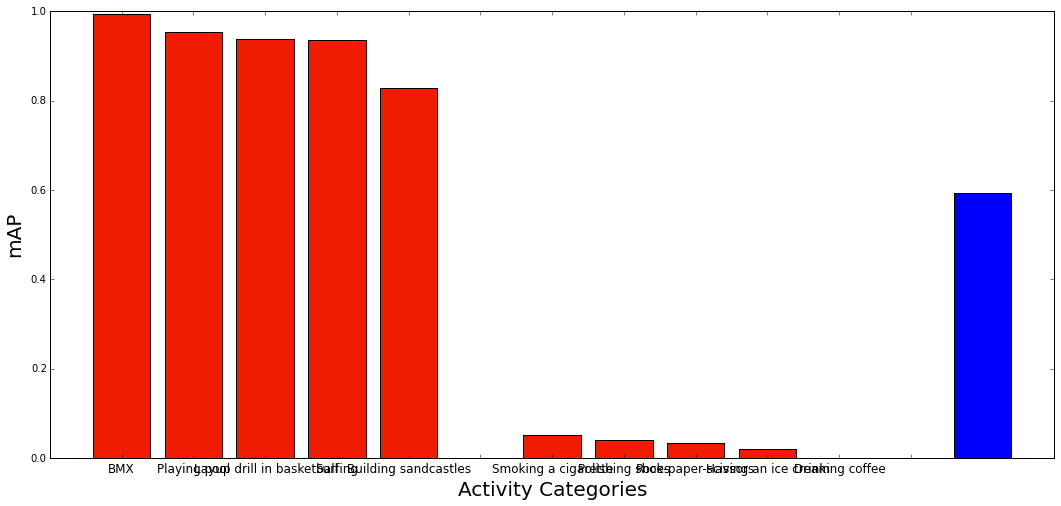
\includegraphics[width=1\linewidth]{img/results/high_low_map_classification}
\end{center}
\caption{Sample of activities with the highest and lowest mAP for the classification task}
\label{fig:map_by_activity_classification}
\end{figure}

\begin{figure}[H]
\begin{center}
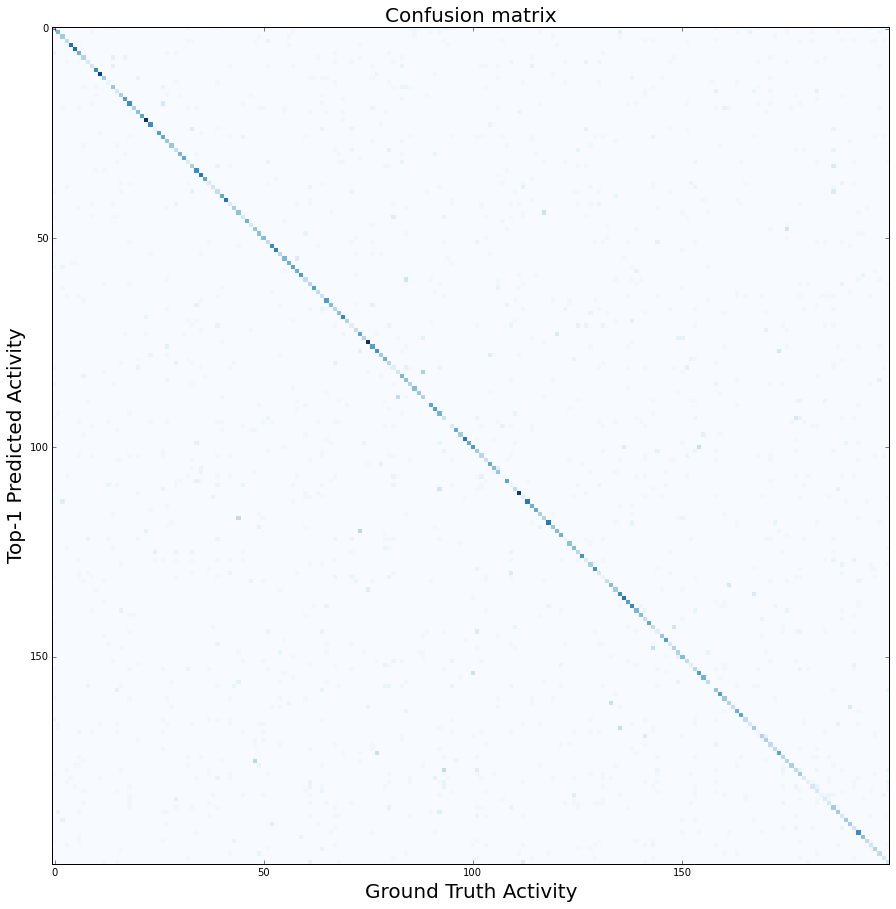
\includegraphics[width=1\linewidth]{img/results/confussion_matrix}
\end{center}
\caption{Confusion matrix of the top-1 activity predicted with the ground truth}
\label{fig:confussion_matrix}
\end{figure}

%%%%%%%%%%%
You think the confusion matrix is good idea to putting on the memory
%%%%%%%%%%%

At the time of submitting the predictions made with the best model for the testing dataset the mAP obtained was of $0.58741$ and the Hi@3 of $0.75548$.

\section{Detection Task}

As the main goal of this project is to obtain a good network to temporally localize activities on videos, it has been compared the results on the detection task of the ActivityNet Challenge for the two architectures proposed. For the basic architecture the network was feed up with video features from the C3D network, while on the feedback architecture, the audio features were concatenated at the input as in classification task improve the results (check Table~\ref{table:classification_by_features}).

%%%%%%%%
How I justify the feedback architecture does not give best results than the basic one?
%%%%%%%%

\begin{table}[H]
\begin{center}
\begin{tabular}{|l|c|}
\hline
Architecture & mAP \\
\hline\hline
Basic Architecture & \bf0.22513 \\
Feedback Architecture &  0.20676 \\
\hline
\end{tabular}
\end{center}
\caption{Best results obtain for the temporal activity localization task in the two architectures}
\label{table:detection_architecture_comparison}
\end{table}

As shows the Table~\ref{table:detection_architecture_comparison} the basic architecture get a slightly better results. The computation of the mean average precision was done doing the same post-processing to the predicted output of the network proposed on this project.

As it was explained on Section~\ref{section:post_processing}, a post-processing was done to the output to achieve a smoother and better temporal prediction of the activities. During this project there were performed some experiments to maximize the prediction precision for different values of $\gamma$ as the activity probability threshold and $k$ as smoothing factor for the mean filter. For different combinations of these variables it was performed the Table~\ref{table:detection_postprocessing_comparison}.

\begin{table}[H]
\begin{center}
\begin{tabular}{|l|c|c|c|}
\hline
$\gamma$ & $k=0$ & $k=5$ & $k=10$ \\
\hline
0.2 & 0.20732 & \bf0.22513 & 0.22136 \\
0.3 & 0.19854 & 0.22077 & 0.22100 \\
0.5 & 0.19035 & 0.21937 & 0.21302 \\
\hline
\end{tabular}
\end{center}
\caption{mAP with an IOU threshold of $0.5$ over validation dataset. Here there is a comparison
between values of $k$ and $\gamma$ on post processing.}
\label{table:detection_postprocessing_comparison}
\end{table}

As can be seen, the best performance was achieved with an activity threshold $\gamma=0.2$ and smoothing filter of $k=5$. The effect of the both of the operations performed after the prediction can be seen on Figures~\ref{fig:smoothing_effect} and~\ref{fig:activty_threshold_effect}. On both figures it is displayed temporally the location of the activity at the ground truth of the video and also the prediction done with the proposed network before and after of each of the post-processing.

\begin{figure}[H]
\begin{center}
%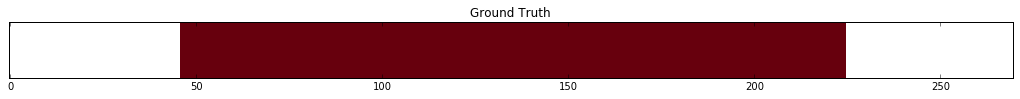
\includegraphics[width=1\linewidth]{img/results/smoothing_effect_1}
%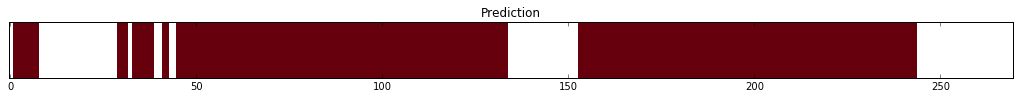
\includegraphics[width=1\linewidth]{img/results/smoothing_effect_2}
%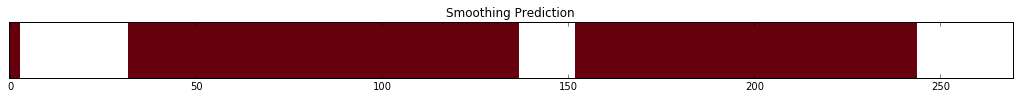
\includegraphics[width=1\linewidth]{img/results/smoothing_effect_3}
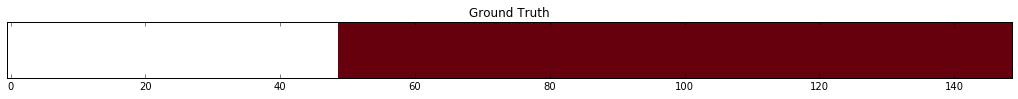
\includegraphics[width=1\linewidth]{img/results/smoothing_effect_4}
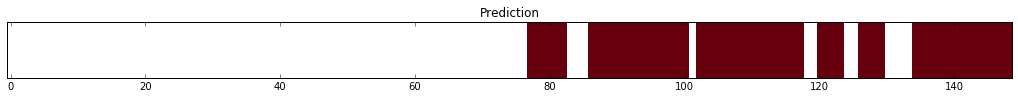
\includegraphics[width=1\linewidth]{img/results/smoothing_effect_5}
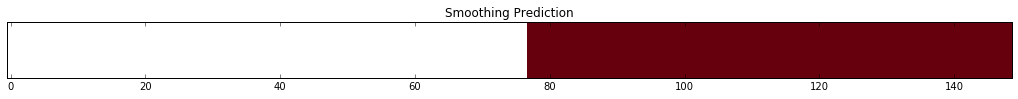
\includegraphics[width=1\linewidth]{img/results/smoothing_effect_6}
\end{center}
\caption{Effect of the mean filter with $k=5$ achieving a smoother activity prediction.}
\label{fig:smoothing_effect}
\end{figure}

\begin{figure}[H]
\begin{center}
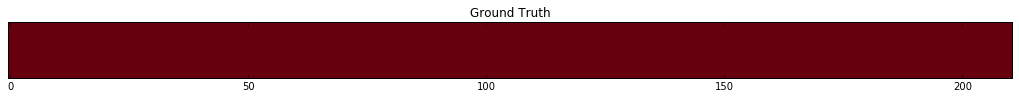
\includegraphics[width=1\linewidth]{img/results/activity_threshold_effect_1}
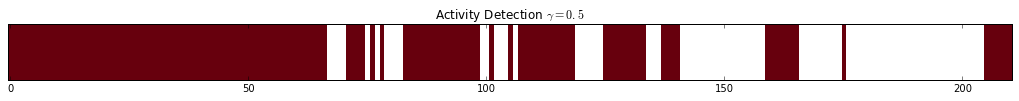
\includegraphics[width=1\linewidth]{img/results/activity_threshold_effect_2}
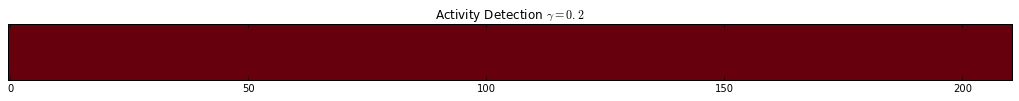
\includegraphics[width=1\linewidth]{img/results/activity_threshold_effect_3}
\end{center}
\caption{}
\label{fig:activty_threshold_effect}
\end{figure}

As it has been done for the classification task, the Average Precision has been computed for the top level activities of the ActivityNet Dataset taxonomy. As can be seen on Table~\ref{table:top_level_detection_ap} and Figure~\ref{fig:top_level_detection_ap} all the top level activities present a similar precision in activity temporal localization except from the category \textit{Personal Care} which does not achieve the half of precision of the rest of top level categories. Also remark that the top level category with highest precision is \textit{Sports, Exercise and Recreation} as happens on the classification task.
%%%%%%
Here will be a figure comparing the prediction with and without smoothing
%%%%%%

\begin{table}[H]
\begin{center}
\begin{tabular}{|r|c|}
\hline
\textbf{Global Activities} & \textbf{AP} \\
\hline\hline
Eating and drinking Activities & 0.25582 \\
Sports, Exercise, and Recreation & 0.30023 \\
Household Activities & 0.26252 \\
Socializing, Relaxing, and Leisure & 0.26060 \\
Personal Care & 0.11234 \\
\hline\hline
\textbf{Global} (mAP) & 0.23830 \\
\hline
\end{tabular}
\end{center}
\caption{Average Precision of activity localization computed for the top level activities of the ActivityNet Dataset. The results are computed over the validation dataset and with a IoU threshold of 0.5.}
\label{table:top_level_detection_ap}
\end{table}

\begin{figure}[H]
\begin{center}
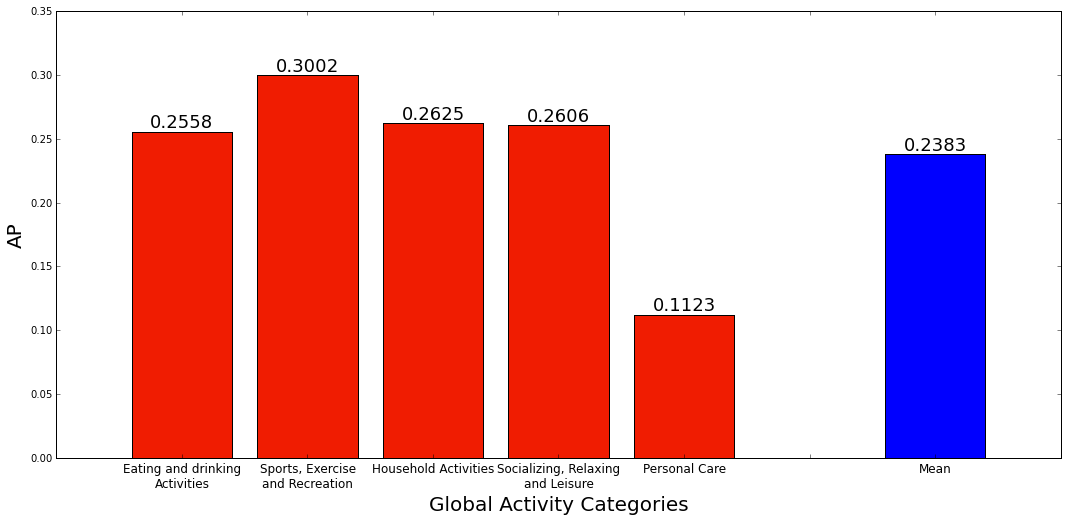
\includegraphics[width=1\linewidth]{img/results/top_activities_detection_ap}
\end{center}
\caption{Representation of the results over the top-level activities}
\label{fig:top_level_detection_ap}
\end{figure}

\begin{figure}[H]
\begin{center}
%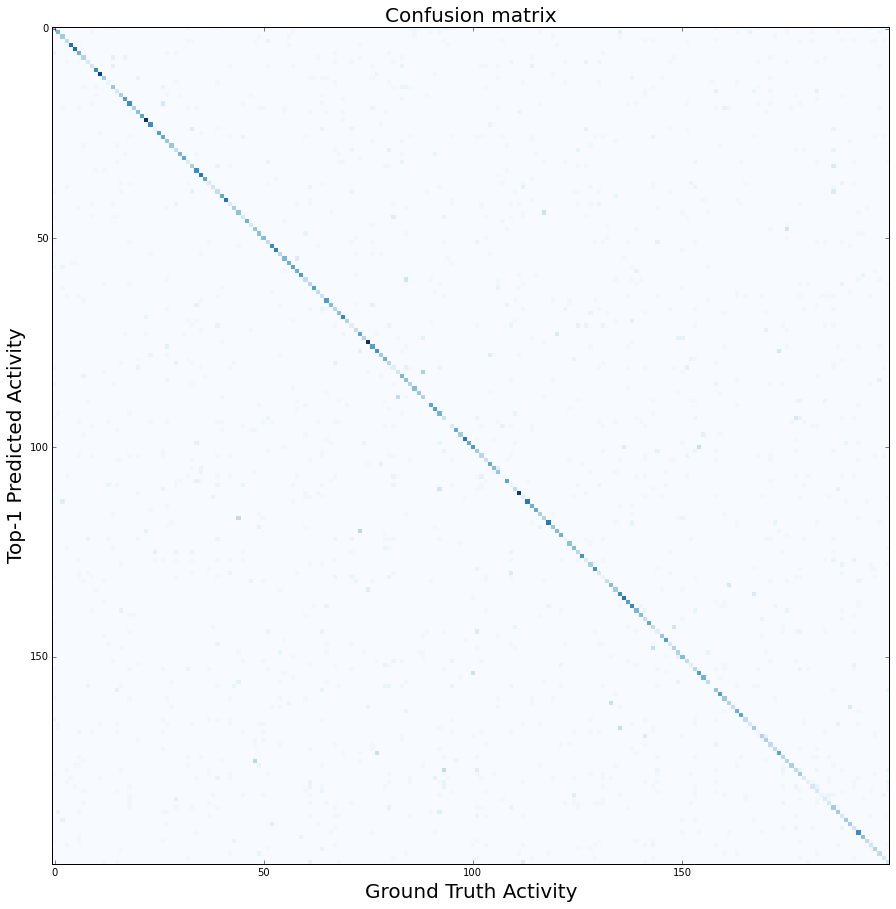
\includegraphics[width=1\linewidth]{img/results/confussion_matrix}
\end{center}
\caption{Activities with higher and lower mAP for the detection task}
\label{fig:map_by_activity_detection}
\end{figure}

%%%%%%%%
I don't know if the previous figure actually putting it
On the other hand I will put a figure ploting the mAP against the IoU asked between 0.1 and 0.5
%%%%%%%%

Plot with multiple IOU and mAP...

\section{Results Visualization}

Here attach some figures about the predictions made by our model.
Spend a whole page with examples of temporal predictions.

Doubt: put the figures as the ground truth and classes predicted in a scale of colours,
or plot only the part of the ground truth that has an activity and also the prediction where the activity is placed as at is computed in the postprocessing to compare?

